\chapter{Renormalization Group}

The renormalization group (RG) is a powerful theoretical framework that allows us to understand the behavior of physical systems at different scales, and in particular to analyze criticality and phase transitions. It provides a unified perspective on the many facets of critical phenomena.

The name ``renormalization group'' is rather misleading: it is a framework in which one applies transformations on a system, but \uline{such transformations do not form a group} in the mathematical sense. However, the name has been kept for historical reasons, since it was first introduced in the context of quantum field theory, where it was used to understand the behavior of quantum fields at different energy scales; now it is used to refer to a more general framework that can be applied to a wide range of systems, and it is associated to a vast set of ideas and techniques that are used to understand critical phenomena in statistical mechanics.\TODO{Add reference to the John Cardy book, chapter 3.}

The renormalization group is based upon the following observation: \textit{critical phenomena are dominated by fluctuations at a scale \(\xi\) which diverges at the critical point; the system thus becomes effectively scale-invariant at criticality}. The idea is to \uline{iteratively modify our description of the system}, eliminating details about the short range correlations at each step, and thus to understand how the system behaves at different scales. In this way, one is eventually left with a simplified description of the system that captures the essential features of the critical behavior through correlations at large scales.

This iterative procedure is called a \textbf{coarse-graining transformation}, and it allows us to understand how the parameters of the system change as we look at it at different scales. It is indeed equivalent to a flow in the space of parameters (space of all possible free energies or actions), which is called the \textbf{action space}, and the \textbf{fixed points} of this flow correspond to critical points of phase transitions. The RG flow allows us to understand the behavior of the system near criticality, and in particular to identify \textit{relevant and irrelevant directions} in the parameter space, associated with the critical exponents that describe the behavior of physical quantities at criticality.

The conceptual framework derived from the RG analysis is very general, and can be implemented in different forms and with different techniques; traditionally, the main distinction is made between \textbf{real space RG} and \textbf{momentum space RG}: the first one is very useful to introduce the framework, as it involves a more intuitive approach; the latter, instead, provides more powerful tools for quantitative computations (for istance, encoding a systematic approach to derive critical exponents below the upper critical dimension).

However, as we said, real space RG is more intuitive and thus we will start by using this approach to revisit the 1D Ising model, which we have already solved, in order to understand how the RG works in a simple case, and then we will introduce the more general framework that can be applied to more complicated systems.

\section{Coarse-Graining in Real Space}

Consider again the 1D Ising model, with Hamiltonian
\[
    H = - J \sum_{i} s_i s_{i+1} - \tilde{h} \sum_i s_i - \tilde{g}N,
\]
were \(J\) is the coupling constant, \(\tilde{h}\) is the external field and we added a constant term \(-\tilde{g}N\) to the Hamiltonian: it does not change the physics of the system, but it will be useful for the RG analysis.

In order to write the partition function, we can introduce the following coefficients:
\[
    \begin{dcases}
        k = \beta J,         \\
        h = \beta \tilde{h}, \\
        g = \beta \tilde{g},
    \end{dcases}
\]
so that we can write the partition function as
\[
    \mathcal{Z} = \sum_{\{s_i\}} e^{k \sum_i s_i s_{i+1}} \, e^{h \sum_i s_i} \, e^{g N}.
\]

Now we have everything described in terms of the spin configurations (microscopic degrees of freedom), but we expect them to carry a lot of unnecessary details, since we are interested in the behavior of the system at larger scales than the microscopic one. The idea is to change our description of the system in terms of \textbf{coarser-grained degrees of freedom}: it naively consists in ``thinning'' the degrees of freedom by summing over some of the spins.

It is easy to understand that this idea can be implemented in different ways, and thus there is not a unique way to perform the coarse-graining transformation, but in general the procedure involves the separation of the system in different blocks and then the definition of a rule to relate the original degrees of freedom to the new ones. We will employ, for the 1D Ising model, the procedure that makes the subsequent computations easier: the so called \textbf{decimation} procedure.

\begin{figure}[H]
    \begin{minipage}{0.55\textwidth}
        \centering
        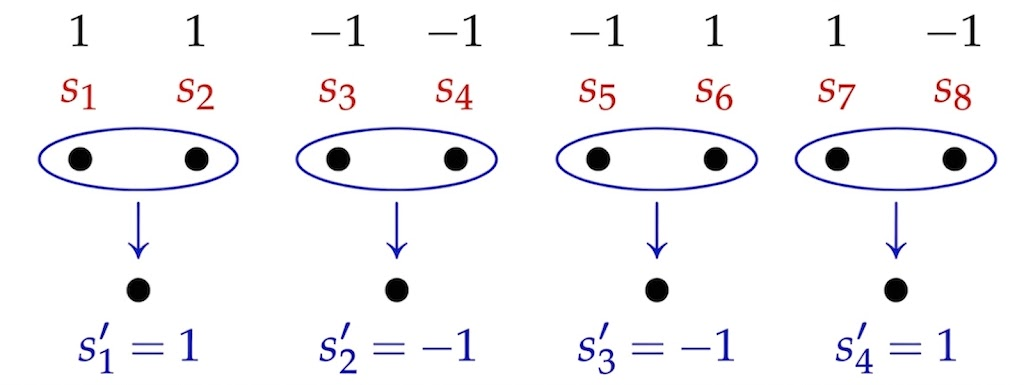
\includegraphics[width=0.9\textwidth]{img/RG_decimation.jpg}
    \end{minipage}
    \hfill
    \begin{minipage}{0.4\textwidth}
        \caption{Decimation procedure for the 1D Ising model: the new coarse-grained degrees of freedom \(s_i^{\prime}\) are defined as the majority of the original ones \((s_i, s_{i+1})\) in each of the two-spins blocks in which we have divided the system.}
    \end{minipage}
\end{figure}

We divide the system into blocks of two spins, and we define the new coarse-grained degrees of freedom \(s_i^{\prime}\) as the majority of the original ones \((s_i, s_{i+1})\) in each block: if the spins are equal, then the majority is well defined, while if they are different, we choose to take the first value of the two, since they are equivalent.\footnote{In other words, we are summing over the odd spins, since we are basically always taking the value of the first spin of the couple.} In this way, we have defined a new set of degrees of freedom that are coarser than the original ones, and we can move on with the RG analysis by writing the partition function in terms of the new degrees of freedom.

In order to do this, let us define the following function of two spins, which will soon come in handy:
\[
    B(s_1,s_2) = k\,s_1 s_2 + \frac{h}{2} (s_1 + s_2) + g.
\]
It can be directly substituted in the expression of the partition function, since the exponent \(-\beta H\) can be written as:
\[
    - \beta H = k \sum_i s_i s_{i+1} + h \sum_i s_i + g N = \sum_i B(s_i, s_{i+1}).
\]
Therefore, the partition function can be written as
\[
    \mathcal{Z} = \sum_{\{s_i\}_{i=1}^N} e^{\sum_{i} B(s_i, s_{i+1})} = \sum_{\{s^{\prime}_i\}_{i=0}^{n'}} \sum_{\{s_i\}_{i=1}^N} e^{\sum_{i} B(s_{i}, s_{i+1})} \prod_{i=0}^{n'} \delta(s_i^{\prime}, s_{2i+1}),
\]
where the delta function enforces the definition of the new degrees of freedom \(s_i^{\prime}\) as the majority of the original ones in each block. Let us highlight that the final product is over the new degrees of freedom, and it spans the new configurations, which are less than the original ones: indeed we defined \(n^{\prime} = \tfrac{N}{2}-1\) since we are considering only the odd-indexed spins in the majority definition we gave for the coarse-graining procedure.

This last identity is not trivial, thus we are going to show it explicitly.
\begin{proof}
    Let us start from a simple case: we have a system with \(N = 4\) spins with periodic boundary conditions, and we want to define the new degrees of freedom as \(s_0^{\prime} = s_1\) and \(s_1^{\prime} = s_3\). The total number of configurations is \(2^4 = 16\)
    \[
        \{s_i\}_{i=1}^4 = \{(1,1,1,1),\,(1,1,1,-1),\,\dots,\, (1,1,-1,-1),\,\dots,\,(-1,-1,-1,-1)\}.
    \]
    We can define \(\mathcal{Z}_{lhs}\) as the microscopical partition function, and \(\mathcal{Z}_{rhs}\) as the coarse-grained one, thus we want to show that \(\mathcal{Z}_{lhs} = \mathcal{Z}_{rhs}\). We can write
    \[
        \begin{aligned}
            \mathcal{Z}_{lhs} = e^{B(1,1) + B(1,1) + B(1,1) + B(1,1)} + e^{B(1,1) + B(1,1) + B(1,-1) + B(-1,1)} \\
            + \dots + e^{B(-1,-1) + B(-1,-1) + B(-1,-1) + B(-1,-1)},
        \end{aligned}
    \]
    while for the new partition function we have to first understand how the coarse-grained degrees of freedom are defined: we have configurations of the form
    \[
        \{s^{\prime}_i\}_{i=0}^1 = \{(1,1),\,(1,-1),\,(-1,1),\,(-1,-1)\},
    \]
    but we have only to consider the configurations of the original spins that are compatible with the definition of the new ones through the delta function. For instance, considering the first configuration \((s_0^{\prime}, s_1^{\prime}) = (1,1)\) we have to consider only the configurations of the original spins such that
    \[
        \delta(s_0^{\prime}, s_1) \delta(s_1^{\prime}, s_3) = \delta(1, s_1) \delta(1, s_3),
    \]
    which means that the original configurations compatible with this definition are only four:
    \[
        \{(1,1,1,1),\,(1,1,1,-1),\,(1,-1,1,1),\,(1,-1,1,-1)\},
    \]
    and thus the contribution to the partition function from this configuration of the new degrees of freedom is
    \[
        \begin{aligned}
            e^{B(1,1) + B(1,1) + B(1,1) + B(1,1)} + e^{B(1,1) + B(1,1) + B(1,-1) + B(-1,1)} \\
            + e^{B(1,-1) + B(-1,1) + B(1,-1) + B(-1,1)} + e^{B(1,-1) + B(-1,1) + B(1,-1) + B(-1,-1)},
        \end{aligned}
    \]
    which is exactly the same contribution we had in the original partition function for the first four configurations of the original spins. We can repeat this procedure for all the other configurations of the new degrees of freedom, and we will find that the contributions to the partition function are exactly the same as in the original one, thus we have \(\mathcal{Z}_{lhs} = \mathcal{Z}_{rhs}\).

    But we can do better than this: we can prove explicity the identity for a generic system with \(N\) spins. We want to prove that
    \[
        \sum_{\{s_i\}_{i=1}^N} e^{\sum_{i} B(s_i, s_{i+1})} = \sum_{\{s^{\prime}_i\}_{i=0}^{n'}} \sum_{\{s_i\}_{i=1}^N} e^{\sum_{i} B(s_{i}, s_{i+1})} \prod_{i=0}^{n'} \delta(s_i^{\prime}, s_{2i+1}).
    \]
    We can switch the order of the sums on the right hand side, since they are finite sums of indipendent variables, thus we can write
    \[
        r.h.s. = \sum_{\{s_i\}_{i=1}^N} \sum_{\{s^{\prime}_i\}_{i=0}^{n'}} e^{\sum_{i} B(s_{i}, s_{i+1})} \prod_{i=0}^{n'} \delta(s_i^{\prime}, s_{2i+1}),
    \]
    then we can take the exponential out of the sum on the new degrees of freedom, since it does not depend on them, and we can write
    \[
        r.h.s. = \sum_{\{s_i\}_{i=1}^N} e^{\sum_{i} B(s_{i}, s_{i+1})} \sum_{\{s^{\prime}_i\}_{i=0}^{n'}} \prod_{i=0}^{n'} \delta(s_i^{\prime}, s_{2i+1}).
    \]
    Now the last sum of products of delta functions is equal to one, since for each configuration of the original spins there is only one configuration of the new degrees of freedom that is compatible with it, thus we have
    \[
        r.h.s. = \sum_{\{s_i\}_{i=1}^N} e^{\sum_{i} B(s_{i}, s_{i+1})} = l.h.s.,
    \]
    which proves the identity.
\end{proof}

After this statistical digression, we can now proceed with the computation of the partition function in terms of the new degrees of freedom. We can write
\[
    \begin{aligned}
        \mathcal{Z} & = \sum_{\{s^{\prime}_i\}_{i=0}^{n'}} \sum_{\{s_i\}_{i=1}^N} e^{\sum_{i} B(s_{i}, s_{i+1})} \prod_{i=0}^{n'} \delta(s_i^{\prime}, s_{2i+1})                                                                                                      \\
                    & = \sum_{\{s^{\prime}_i\}_{i=0}^{n'}} \sum_{\{s_i\}_{i=1}^N} e^{ \sum_{i=0}^{\frac{N}{2}-1} \left( B(s_{2i+1}, s_{2i+2}) + B(s_{2i+2}, s_{2i+3}) \right) } \prod_{i=0}^{n'} \delta(s_i^{\prime}, s_{2i+1})                                       \\
                    & = \sum_{\{s^{\prime}_i\}_{i=0}^{n'}} \sum_{\{s_{2i+2}\}_{i=0}^{n^{\prime}}} e^{\sum_{i=0}^{n^{\prime}} B(s_i^{\prime}, s_{2i+2}) + B(s_{2i+2}, s_{i+1}^{\prime})} = \sum_{\{s^{\prime}_i\}_{i=0}^{n'}} e^{-\beta H^{\prime}[\{s_i^{\prime}\}]},
    \end{aligned}
\]
where we have defined \(H^{\prime}\) as a new Hamiltonian that depends on the new degrees of freedom; now we can further simplify the expression as follows:
\[
    \begin{aligned}
        e^{-\beta H^{\prime}[\{s_i^{\prime}\}]} & = \sum_{\{s_{2i+2}\}_{i=0}^{n^{\prime}}} e^{\sum_{i=0}^{n^{\prime}} B(s_i^{\prime}, s_{2i+2}) + B(s_{2i+2}, s_{i+1}^{\prime})}  \\
                                                & = \prod_{i=0}^{n^{\prime}} \left[ \sum_{s_{2i+2} = \pm 1} e^{B(s_i^{\prime}, s_{2i+2}) + B(s_{2i+2}, s_{i+1}^{\prime})} \right] \\
                                                & = e^{\sum_{i=0}^{n^{\prime}} B^{\prime} (s_i^{\prime}, s_{i+1}^{\prime})},
    \end{aligned}
\]
where we have defined the new \(B^{\prime}\) as the function satisfying the following identity:
\[
    e^{B^{\prime} (s_1^{\prime}, s_2^{\prime})} = \sum_{s = \pm 1} e^{B(s_1^{\prime}, s) + B(s, s_2^{\prime})}.
\]
Since this function must be symmetric under the exchange of \(s_1^{\prime}\) and \(s_2^{\prime}\), it can be proven rigorously that its most general form is
\[
    B^{\prime} (s_1^{\prime}, s_2^{\prime}) = k^{\prime} s_1^{\prime} s_2^{\prime} + \frac{h^{\prime}}{2} (s_1^{\prime} + s_2^{\prime}) + g^{\prime},
\]
where \(k^{\prime}\), \(h^{\prime}\) and \(g^{\prime}\) are new parameters that depend on the original ones, and they are implicitly defined by the above identity.

This is a crucial step in the RG analysis: we have shown that after the coarse-graining transformation, the partition function can be written as
\[
    \mathcal{Z} = \sum_{\{s^{\prime}_i\}_{i=0}^{n'}} e^{-\beta H^{\prime}[\{s_i^{\prime}\}]},
\]
where the new Hamiltonian has the same form as the original one, but with different parameters
\[
    - \beta H^{\prime}[\{s_i^{\prime}\}] = \sum_{i=1}^{N/2} B^{\prime} (s_i^{\prime}, s_{i+1}^{\prime}) = k^{\prime} \sum_{i=1}^{N/2} s_i^{\prime} s_{i+1}^{\prime} + h^{\prime} \sum_{i=1}^{N/2} s_i^{\prime} + g^{\prime} \frac{N}{2},
\]
which means we have \textit{coarse-grained} the description of the system
\[
    \begin{aligned}
        \{s_i\}_{i=1}^{N} \quad & \to \quad \{s_i^{\prime}\}_{i=0}^{n'},          \\
        (k, h, g) \quad         & \to \quad (k^{\prime}, h^{\prime}, g^{\prime}).
    \end{aligned}
\]
In the thermodinamic limit \(N \to \infty\) this transformation corresponds to a flow in the space of parameters, which is a way of thinking about the RG transformation that we will extensively discuss in the following.

To sum up, we have shown that the partition function of the original system can be written as the partition function of a new system with the same form of the Hamiltonian, but with different parameters: we started from the original hamiltonian
\[
    - \beta H = k \sum_i s_i s_{i+1} + h \sum_i s_i + g N = \sum_i B(s_i, s_{i+1}),
\]
inside the exponential of the partition function, and through the coarse-graining transformation we have derived a new hamiltonian
\[
    - \beta H^{\prime} = k^{\prime} \sum_i s_i^{\prime} s_{i+1}^{\prime} + h^{\prime} \sum_i s_i^{\prime} + g^{\prime} \frac{N}{2} = \sum_i B^{\prime}(s_i^{\prime}, s_{i+1}^{\prime}),
\]
and in this new description in terms of the ``renormalized'' Hamiltonian, depending upon the new parameters \(k^{\prime}\), \(h^{\prime}\) and \(g^{\prime}\). In this case, the functional form of the Hamiltonian (and thus the partition function) is preserved, but the parameters are changed, and they are implicitly defined by the identity in equation (?)\TODO{add reference}, which explicitly reads
\[
    e^{k^{\prime} s_1^{\prime} s_2^{\prime} + \frac{h^{\prime}}{2} (s_1^{\prime} + s_2^{\prime}) + g^{\prime}} = \sum_{s = \pm 1} e^{k s (s_1^{\prime} + s_2^{\prime}) + \frac{h}{2} (s_1^{\prime} + s_2^{\prime}) + hs + 2g}.
\]
It is now convenient to employ the following change of variables:
\[
    \begin{dcases}
        x = e^k, \\
        y = e^h, \\
        z = e^g,
    \end{dcases} \qquad \begin{dcases}
        x^{\prime} = e^{k^{\prime}}, \\
        y^{\prime} = e^{h^{\prime}}, \\
        z^{\prime} = e^{g^{\prime}}.
    \end{dcases}
\]
We have then four possible choices for \((s^{\prime}_1,\,s^{\prime}_2) = (\pm 1,\, \pm 1)\), all of which need to satisfy the above identity, thus we have the following system of equations:
\[
    \begin{aligned}
        (+1,\,+1) \quad & \implies \quad x^{\prime} y^{\prime} z^{\prime} = z^2 y (x^2 y + x^2 y^{-1}),                \\
        (+1,\,-1) \quad & \implies \quad (x^{\prime})^{-1} z^{\prime} = z^2 (y + y^{-1}),                              \\
        (-1,\,+1) \quad & \implies \quad (x^{\prime})^{-1} z^{\prime} = z^2 (y + y^{-1}),                              \\
        (-1,\,-1) \quad & \implies \quad x^{\prime} (y^{\prime})^{-1} z^{\prime} = z^2 y^{-1} (x^{-2} y + x^2 y^{-1}).
    \end{aligned}
\]
The system is determined, since we have three unknowns \(x^{\prime}\), \(y^{\prime}\) and \(z^{\prime}\) and three independent equations (the second and the third one are the identical). With simple algebra we can find the solution
\[
    \begin{dcases}
        (z^{\prime})^4 = z^8 (x^2 y + x^{-2} y^{-1})(x^{-2} y + x^{2} y^{-1}) (y + y^{-1})^2, \\
        (y^{\prime})^2 = y^2 \frac{x^2 y + x^{-2} y^{-1}}{x^{-2} y + x^{2} y^{-1}},           \\
        (x^{\prime})^4 = \frac{(x^2 y + x^{-2} y^{-1})(x^{-2} y + x^{2} y^{-1})}{(y + y^{-1})^2},
    \end{dcases}
\]
which provides, after taking the logarithm, the \textbf{RG flow equations} for the parameters \(k\) and \(h\):
\[
    \begin{dcases}
        g^{\prime} = 2g + \delta g(k, h), \\
        h^{\prime} = h + \delta h(k, h),  \\
        k^{\prime} = k^{\prime} (k, h)
    \end{dcases}
\]
where \(\delta g\), \(\delta h\) and \(k^{\prime} (k, h)\) are implicitly defined by the above equations. \uline{This flow equations describe how the parameters of the Hamiltonian change in the \textbf{action space} (or \textit{free energy space}) as we perform a \textbf{coarse-graining transformation}}. The fixed points of this flow correspond to scale-invariant theories, which are often associated with critical points of phase transitions.

\begin{remark}
    When we write the Hamiltonian, if we assume directly that \(N \to \infty\), the system has an infinite number of degrees of freedom, and the RG transformation is from an infinite-dimensional space to itself, which is not very useful. Instead, we can consider a finite system with \(N\) sites, and then take the limit \(N \to \infty\) at the end of the calculation.

    We are speaking about a space of parameters, not a space of configurations, so the RG transformation is from a finite-dimensional space to itself, which is more manageable.
\end{remark}

Notice how during the RG transformation, lenghts in the system are actually rescaled: in the original microscopic description, the distance between two neighboring spins is one, while in the new description, the distance between two neighboring can be two (as an example, \(s_1\) and \(s_3\) are not neighbors, but the new spins \(s_0^{\prime}\) and \(s_2^{\prime}\), defined by the previous ones, are neighbors). Thus, spins which where separated by a distance \(R\) in the original lattice are now effevtively separated by a distance \(R/2\) in the new lattice, and thus the RG transformation is also a \textbf{length rescaling} transformation.

\subsection{Recursion Relations and Flow Diagrams}

The previous set of equations is also called the \textbf{RG recursion relations} for the parameters of the Hamiltonian, and they can be used to understand how the system behaves at different scales. In particular, they allow us to identify the fixed points of the RG flow, which correspond to scale-invariant theories, and thus to critical points of phase transitions.

Although the Ising model is a very simple model, the RG analysis is not trivial, and it can be quite involved for more complicated models. However, the presented approach to compute the partition function already reveals the essential and recurring themes of the RG analysis.

In general one proceeds as follows:
\begin{enumerate}
    \item \textbf{Coarse-graining} or ``thinning'' of the degrees of freedom: we define new degrees of freedom that are coarser than the original ones, and we write the partition function in terms of these new degrees of freedom.
    \item \textbf{Lenght rescaling}: after the coarse-graining transformation, the new degrees of freedom are defined on a lattice with a different spacing, thus we need to rescale the lengths in order to compare the new system with the original one.
    \item Derivation of new \textbf{renormalized Hamiltonian}: after the coarse-graining and the length rescaling, we can write the partition function in terms of a new Hamiltonian that has the same form as the original one, but with different parameters.
\end{enumerate}
We will soon come back to these steps to clarify and state them in a more general and rigorous way, but for now we can already see how they work in the case of the 1D Ising model. However, this is the essential procedure to obtain the RG flow equations for the parameters of the Hamiltonian, which are the main tool to derive predictions about the critical behavior of the system (existence of phase transitions, critical exponents, etc.).

\subsubsection{Ising RG Flow: No External Field}

Now let us set \(h=0\), which implies \(y=1\), and see how the RG flow looks like in the \((k, h)\) plane. The flow equations give us
\[
    y^{\prime} = \frac{x^2 + x^{-2}}{x^2 + x^{-2}} = 1 \implies h^{\prime} = 0,
\]
and we can write the recursion relation for \(k\) (from \((x^{\prime})^4\)) as
\[
    e^{4k^{\prime}} = \left(\frac{e^{2k} + e^{-2k^{\prime}}}{2}\right)^2 \quad \implies \quad k^{\prime} = \frac{1}{2} \ln \left(\cosh(2k)\right).
\]
This recursion relation has two fixed points, which can be found by setting \(k^{\prime} = k\):
\[
    k = \frac{1}{2} \ln \left(\cosh(2k)\right) \quad \implies \quad k = 0 \quad \text{or} \quad k = +\infty.
\]
This is because the function \(f(k) = \frac{1}{2} \ln \left(\cosh(2k)\right)\) is a monotonically increasing function of \(k\) (the hyperbolic cosine is almost a parabola and its logarithm is also monotonically increasing for \(k > 0\)) that starts from \(f(0) = 0\) and diverges as \(k \to +\infty\). Thus, the only points where \(f(k) = k\) are at \(k = 0\) and \(k = +\infty\).

The fixed points are the only candidates for critical points (where the system can undergo a phase transition), since they are the only points where the system is scale-invariant.

The first one is unstable, while the second one is stable:
\begin{itemize}
    \item At \(k = 0\), we have \(\beta = 0\), and thus an infinite temperature \(T \to \infty\): it is a \textbf{stable} fixed point. If we perturb it slightly, for a small \(k\), we have
          \[
              k^{\prime} = \frac{1}{2} \ln \left(\cosh(2k)\right) \approx \frac{1}{2}\ln(1 + \left(\tfrac{2k}{2}\right)^2) \approx k^2 < k,
          \]
          which means that the flow is pushing towards \(k = 0\): the system is driven towards the infinite temperature limit, where it is disordered. This is also called \textbf{sink} or \textbf{attractor}.
    \item At \(k = \infty\), we have \(\beta \to \infty\), and thus a zero temperature \(T \to 0\): it is an \textbf{unstable} fixed point. If we perturb it slightly, for a large \(k\), we have
          \[
              k^{\prime} = \frac{1}{2} \ln \left(\cosh(2k)\right) \approx \frac{1}{2} \ln \left(\frac{e^{2k}}{2}\right) = k - \ln 2 < k,
          \]
          which means that the flow is pushing towards \(k = 0\) and an infinite temperature: indeed, a perturbation to the large coupling constant \(k\) will make it smaller, effectively driving away the system from the zero temperature limit, where it is ordered.
\end{itemize}

In this case, the only critical point is at \(k = 0\), which corresponds to the infinite temperature limit, where the system is disordered. The other fixed point at \(k = \infty\) corresponds to the zero temperature limit, where the system is ordered, but it is unstable, since any perturbation will drive the system away from it. Thus, there is no phase transition at finite temperature in the 1D Ising model, and the system is always disordered for any finite temperature.

\begin{figure}[H]
    \centering
    \begin{minipage}{0.8\textwidth}
        \centering
        \begin{tikzpicture}[
                flow/.style={
                        decoration={
                                markings,
                                mark=at position 0.08 with {\arrow[blue, line width=1.5pt]{<}},
                                mark=at position 0.13 with {\arrow[blue, line width=1.5pt]{<}},
                                mark=at position 0.22 with {\arrow[blue, line width=1.5pt]{<}},
                                mark=at position 0.50 with {\arrow[blue, line width=1.5pt]{<}},
                                mark=at position 0.75 with {\arrow[blue, line width=1.5pt]{<}},
                                mark=at position 0.88 with {\arrow[blue, line width=1.5pt]{<}},
                                mark=at position 0.93 with {\arrow[blue, line width=1.5pt]{<}},
                            },
                        postaction={decorate}
                    }
            ]
            \draw[thick, flow] (0,0) -- (10,0);

            \fill[red!80!black] (0,0) circle (4pt);
            \fill[red!80!black] (10,0) circle (4pt);

            \node[below=8pt] at (0,0) {$K=0$};
            \node[below=8pt] at (10,0) {$K=+\infty$};

        \end{tikzpicture}
    \end{minipage}
    \begin{minipage}{0.8\textwidth}
        \centering
        \begin{tikzpicture}[
                flow/.style={
                        decoration={
                                markings,
                                mark=at position 0.08 with {\arrow[blue, line width=1.5pt]{>}},
                                mark=at position 0.13 with {\arrow[blue, line width=1.5pt]{>}},
                                mark=at position 0.25 with {\arrow[blue, line width=1.5pt]{>}},
                                mark=at position 0.50 with {\arrow[blue, line width=1.5pt]{>}},
                                mark=at position 0.75 with {\arrow[blue, line width=1.5pt]{>}},
                                mark=at position 0.88 with {\arrow[blue, line width=1.5pt]{>}},
                                mark=at position 0.93 with {\arrow[blue, line width=1.5pt]{>}},
                            },
                        postaction={decorate}
                    }
            ]

            \draw[thick, flow] (0,0) -- (10,0);

            \fill[red!80!black] (0,0) circle (4pt);
            \fill[red!80!black] (10,0) circle (4pt);

            \node[below=8pt] at (0,0) {$T=0$};
            \node[below=8pt] at (10,0) {$T=+\infty$};
        \end{tikzpicture}
    \end{minipage}
    \caption{One-dimensional renormalization group (RG) flow diagrams. The upper figure depicts the flow of the coupling constant $K$ towards the trivial fixed point at $K=0$. The lower figure shows the equivalent flow parameterized by temperature $T$, where the system is driven away from the unstable critical point at $T=0$ towards the stable high-temperature limit at $T=+\infty$.}
\end{figure}

Thus the initial problem \(\mathcal{Z}(\beta, h=0) \) is recursively mapped onto new ones \(\mathcal{Z}^{\prime}(\beta^{\prime}, h=0)\), \(\mathcal{Z}^{\prime\prime}(\beta^{\prime\prime}, h=0)\), etc., which by construction have to be all numerically equal to the original one, but with different parameters. The flow of the parameters under the RG transformation allows us to understand the behavior of the system at different scales, and in particular to identify the critical points and the nature of the phase transitions. So under repeated RG transformations, any initial ``hard'' Hamiltonian (depending upon a generic \(\beta\)) is mapped onto a new simpler one arbitrarily closer to the stable fixed point \(\beta \sim 0\). Furthermore we got to identify some fixed points of the flow, which are the only candidates for critical points.

\subsubsection{Ising RG Flow: External Field}

Going beyond and introducing an external field \(h \neq 0\) we can also derive a \textbf{flow diagram} for generic values of \(k\) and \(h\), which is a graphical representation of the RG flow in the parameter space. The flow diagram allows us to visualize how the parameters evolve under the RG transformation, and to identify the fixed points and their stability properties.

\begin{figure}[H]
    \begin{minipage}{0.6\textwidth}
        \centering
        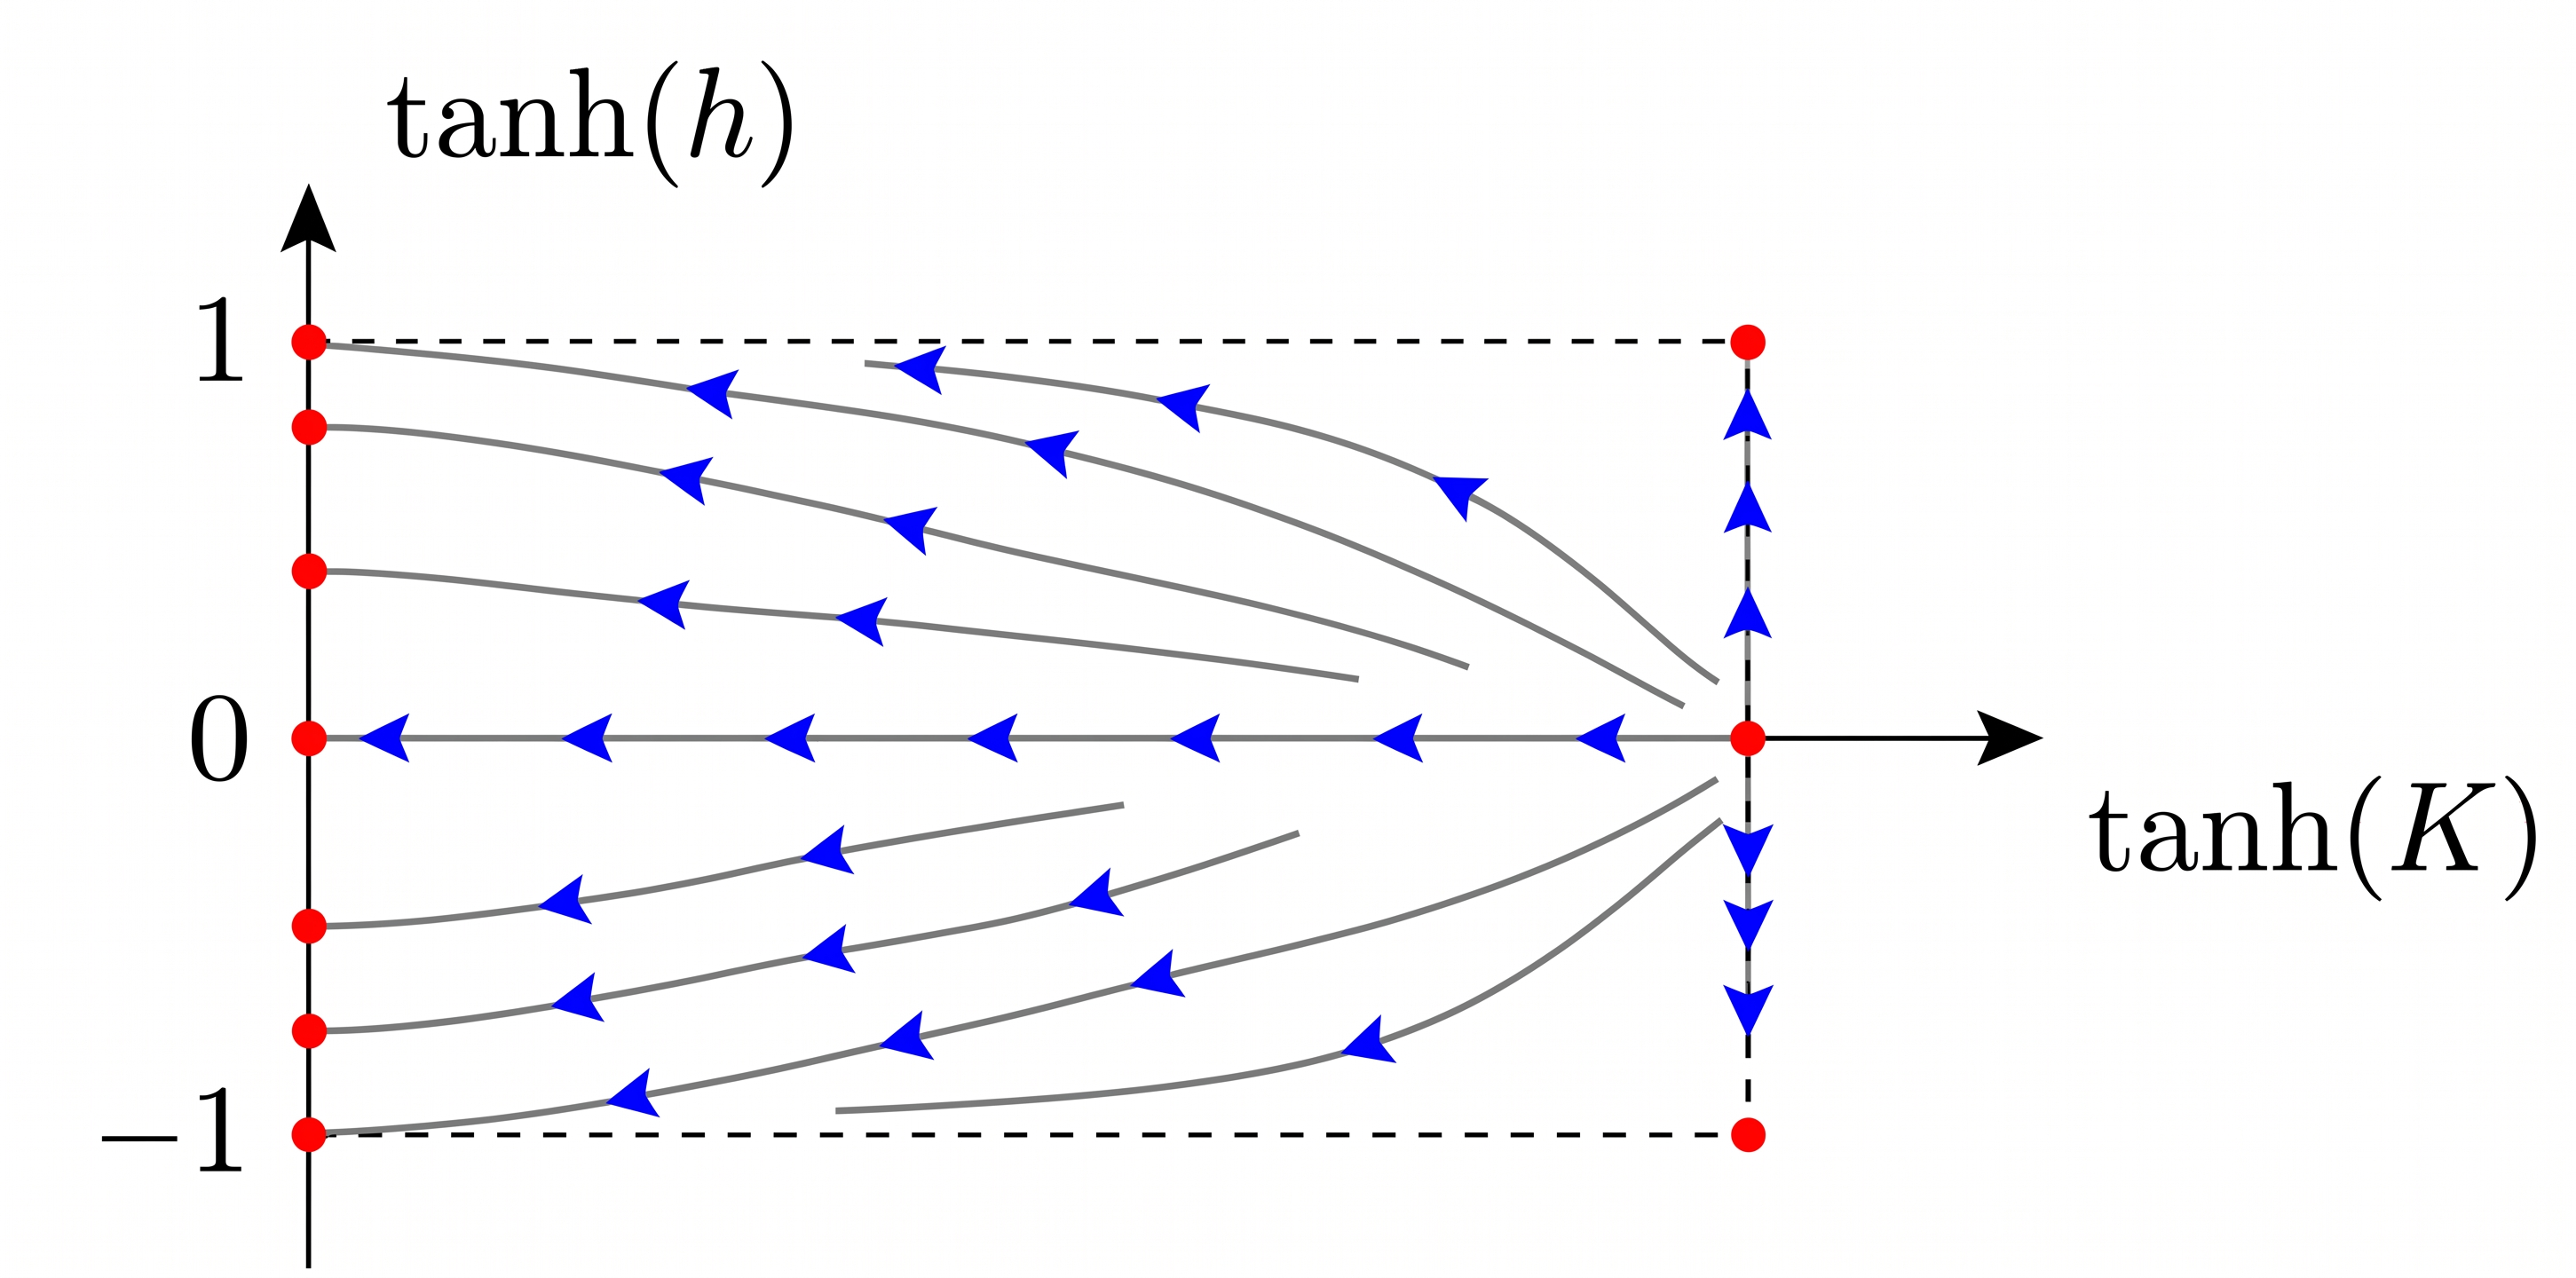
\includegraphics[width=0.8\textwidth]{img/RG_flow_temporary.png}
    \end{minipage}
    \hfill
    \begin{minipage}{0.35\textwidth}
        \caption{Flow diagram for the 1D Ising model in the \((k, h)\) plane. The flow lines indicate how the parameters \(k\) and \(h\) evolve under the RG transformation.}
    \end{minipage}
\end{figure}

In the precence of an external field, the flow diagram becomes more complex, but we can still identify the fixed points and their stability properties. All points in the parameter space flow towards the stable fixed points at \(k = 0\) and arbitrary \(h\), which corresponds to the disordered phase with independent and uncorrelated spins (\(\xi=0\) in this case).

\subsection{Linearization and Scaling Form}

It is now time to investigate how the analysis of the RG flow allows us to obtain predictions about the behavior of physical quantities near the fixed points, the only candidates for critical points. In particular, the 1D Ising model does not have a phase transition at finite temperature, making this study rather trivial, but the method we are going to use is general and can be applied to more complicated models, where the RG flow can be more complex and the fixed points can have different stability properties.

Thus we can start by linearizing the flow equations around the fixed points since we are interested in the behavior near these. Let us consider in particular \(T \sim 0\) and \(h \sim 0\), corresponding to \(y \sim 1\) and \(x \to \infty\). We can write
\[
    \begin{dcases}
        (x^{\prime})^4 \simeq \frac{x^4}{4}, \\
        (y^{\prime})^2 \simeq y^2 \frac{x^2 y}{x^2 y^{-1}} = y^4,
    \end{dcases} \quad \implies \quad \begin{dcases}
        e^{-k^{\prime}} = \sqrt{2} e^{-k}, \\
        h' = 2 h.
    \end{dcases}
\]
After each RG iteration, the correlation length gets divided by two, and therefore, we can write \(\xi\) as a function of \(e^{-k}\) and \(h\):
\[
    \xi = \xi(k,h) \to \frac{\xi(k,h)}{2} = \xi(k^{\prime}, h^{\prime}),
\]
where the equality is due to the fact that the partition function is invariant under the RG transformation, thus the correlation length must be invariant as well. This is a crucial point: the RG transformation is a change of variables in the partition function, which does not change its value, thus any physical quantity derived from it must be invariant under the RG transformation.

Thus we have the following identity for the correlation length:
\[
    \frac{1}{2} \xi(e^{-k}, h) = \xi(\sqrt{2} e^{-k}, 2h),
\]
which after \(\ell\) RG iterations becomes
\[
    \xi(e^{-k}, h) = 2^{\ell} \xi(2^{\ell/2} e^{-k}, 2^{\ell} h).
\]
Now if we chose \(\ell\) such that
\[
    2^{\ell/2}e^{-k} = 1 \quad \implies \quad 2^\ell = e^{2k},
\]
since we are interested in the behavior near \(k \to \infty\) (or \(T \to 0\)) and we want to keep the first argument of the correlation length fixed, we obtain the \textbf{scaling form} of the correlation length:
\[
    \xi(e^{-k}, h) = e^{2k} \xi(1, e^{2k} h) = e^{2k} g_\xi(e^{2k} h),
\]
where \(g_\xi\) is a scaling function that depends on the combination \(e^{2k} h\). This is the most non trivial result of the RG analysis: we are rewriting a new hamiltonian with new parameters, but the partition function is the same, and thus the correlation length is the same. This is what allowed us to derive the scaling form of the correlation length.

Now setting \(h \to 0\) to study the behavior of the correlation length at zero magnetic field, we can treat \(g_\xi(0)\) as a constant, and we obtain
\[
    \xi(e^{-k}, 0) \sim e^{2k} \sim e^{2\beta J} \sim e^{\frac{2J}{k_B T}},
\]
which is the well-known result for the correlation length of the 1D Ising model at zero magnetic field. This shows how the RG analysis allows us to derive the scaling behavior of physical quantities near critical points, and in this case, it confirms that there is no phase transition at finite temperature, since the correlation length diverges only as \(T \to 0\). We had to postulate the scaling form of the correlation length, but now we have an hint the RG ideas are adequate to derive the scaling form of physical quantities near critical points, and in particular to understand the behavior of the correlation length as a function of the parameters of the system.
